\documentclass[tikz,border=10pt]{standalone}
\usepackage{tikz}
\usetikzlibrary{shapes.geometric,positioning,calc,arrows.meta}

\definecolor{entityfill}{HTML}{C8BAE7}
\definecolor{supertypefill}{HTML}{B5A1E0}
\definecolor{diamondfill}{HTML}{F9D053}
\definecolor{ink}{HTML}{16232C}
\definecolor{linegray}{HTML}{4D4D4D}

\begin{document}
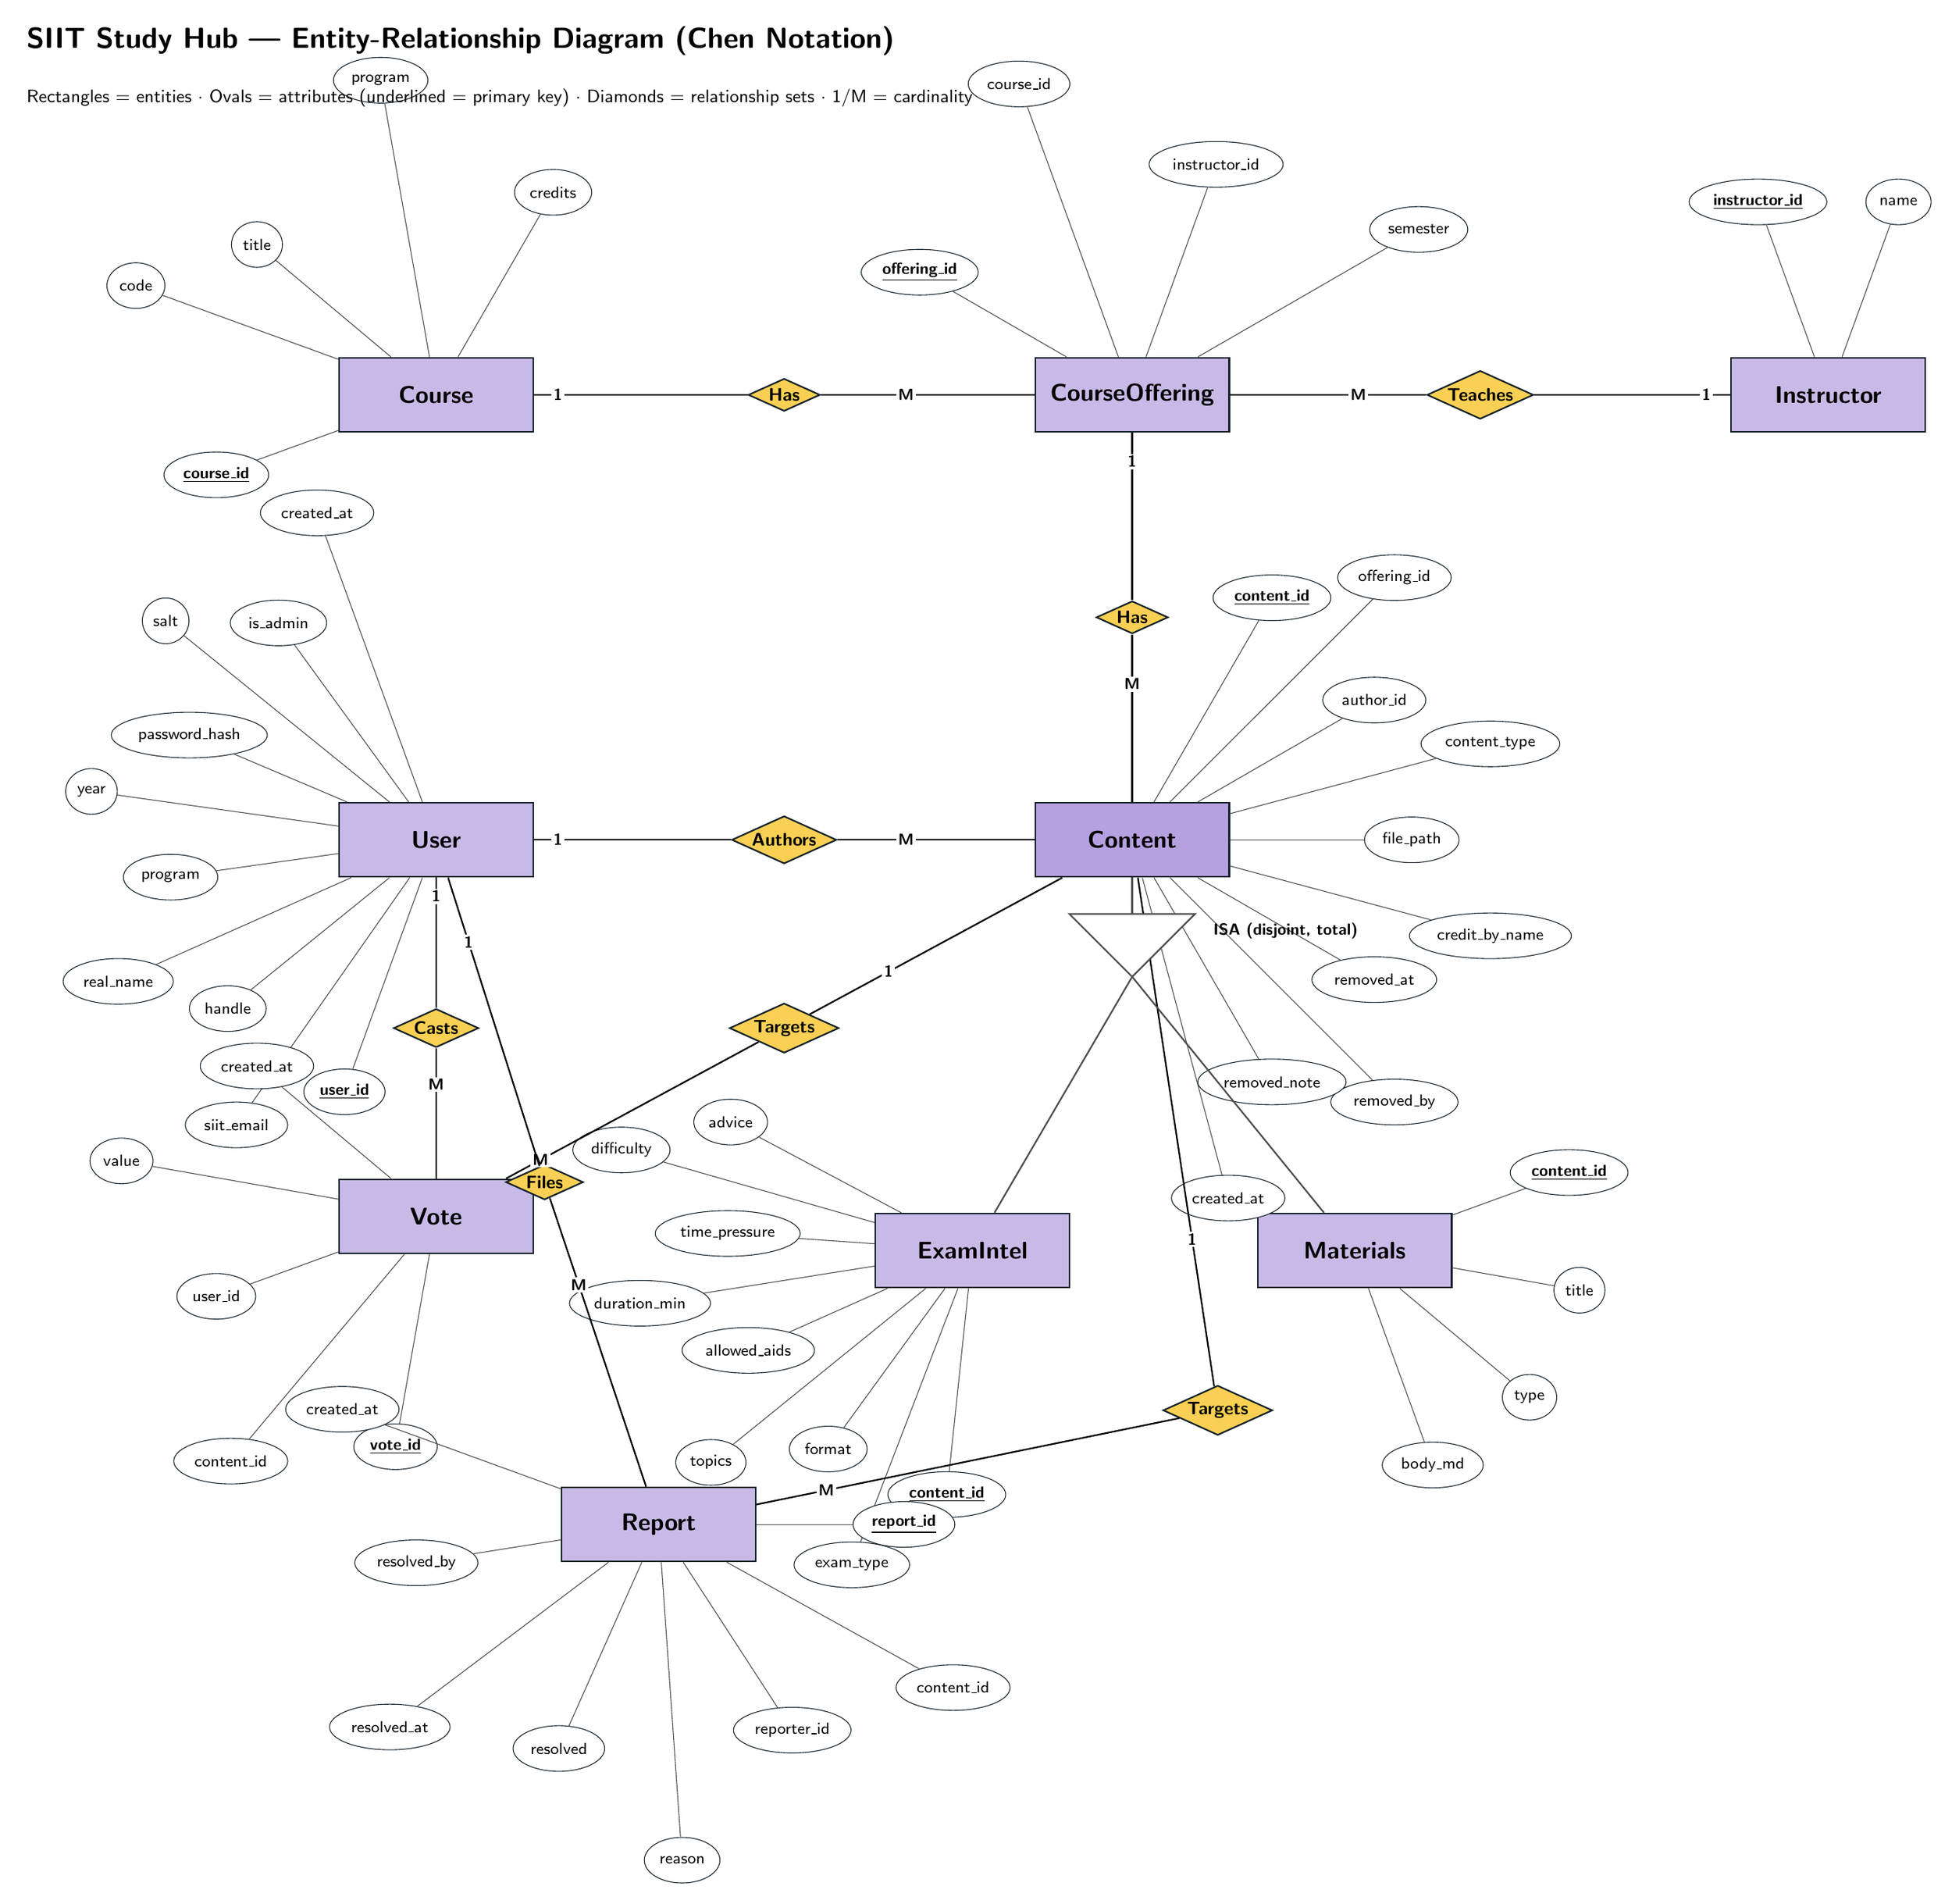
\begin{tikzpicture}[
  >=Stealth,
  every node/.style={font=\sffamily},
  entity/.style={rectangle, draw=ink, thick, fill=entityfill, minimum width=34mm, minimum height=13mm, align=center, font=\sffamily\bfseries\large},
  supertype/.style={entity, fill=supertypefill},
  attr/.style={ellipse, draw=ink, fill=white, inner sep=2pt, font=\sffamily\footnotesize, minimum height=8mm},
  pk/.style={attr, font=\sffamily\footnotesize\bfseries},
  rel/.style={diamond, draw=ink, thick, fill=diamondfill, aspect=2.2, inner sep=1pt, align=center, font=\sffamily\bfseries\small},
  card/.style={font=\sffamily\bfseries\footnotesize, fill=white, inner sep=1pt},
  isaline/.style={draw=linegray, thick},
]

% ---------- helper: attribute placed by polar offset from an entity ----------
% \attrnode{entity}{angle}{radius}{node name}{label}
\newcommand{\attrnode}[5]{%
  \node[attr] (#4) at ($(#1)+(#2:#3)$) {#5};
  \draw[linegray] (#1) -- (#4);
}
\newcommand{\pkattrnode}[5]{%
  \node[pk] (#4) at ($(#1)+(#2:#3)$) {\underline{#5}};
  \draw[linegray] (#1) -- (#4);
}

% ================= ENTITIES =================
\node[entity] (Course) at (7.8,-5.0) {Course};
\node[entity] (CourseOffering) at (20.0,-5.0) {CourseOffering};
\node[entity] (Instructor) at (32.2,-5.0) {Instructor};
\node[entity] (User) at (7.8,-12.8) {User};
\node[supertype] (Content) at (20.0,-12.8) {Content};
\node[entity] (ExamIntel) at (17.2,-20.0) {ExamIntel};
\node[entity] (Materials) at (23.9,-20.0) {Materials};
\node[entity] (Vote) at (7.8,-19.4) {Vote};
\node[entity] (Report) at (11.7,-24.8) {Report};

% ================= ATTRIBUTES =================
% NOTE: angles are negated relative to the original design sketch, because
% TikZ's polar coordinates are counter-clockwise (y-up) while the sketch
% used a clockwise/y-down convention. Radii are also scaled up ~1.8x to
% keep proper clearance around the larger (34mm) entity boxes.

% Course (5)
\pkattrnode{Course}{200}{4.1}{a-course-id}{course\_id}
\attrnode{Course}{160}{5.6}{a-course-code}{code}
\attrnode{Course}{140}{4.1}{a-course-title}{title}
\attrnode{Course}{100}{5.6}{a-course-program}{program}
\attrnode{Course}{60}{4.1}{a-course-credits}{credits}

% CourseOffering (4)
\pkattrnode{CourseOffering}{150}{4.3}{a-co-id}{offering\_id}
\attrnode{CourseOffering}{110}{5.8}{a-co-courseid}{course\_id}
\attrnode{CourseOffering}{70}{4.3}{a-co-instrid}{instructor\_id}
\attrnode{CourseOffering}{30}{5.8}{a-co-semester}{semester}

% Instructor (2)
\pkattrnode{Instructor}{110}{3.6}{a-instr-id}{instructor\_id}
\attrnode{Instructor}{70}{3.6}{a-instr-name}{name}

% User (10)
\pkattrnode{User}{250}{4.7}{a-user-id}{user\_id}
\attrnode{User}{235}{6.1}{a-user-email}{siit\_email}
\attrnode{User}{219}{4.7}{a-user-handle}{handle}
\attrnode{User}{204}{6.1}{a-user-realname}{real\_name}
\attrnode{User}{188}{4.7}{a-user-program}{program}
\attrnode{User}{172}{6.1}{a-user-year}{year}
\attrnode{User}{157}{4.7}{a-user-pwhash}{password\_hash}
\attrnode{User}{141}{6.1}{a-user-salt}{salt}
\attrnode{User}{126}{4.7}{a-user-isadmin}{is\_admin}
\attrnode{User}{110}{6.1}{a-user-created}{created\_at}

% Content (10, supertype) -- fanned to the right, clear of the ISA triangle below
\pkattrnode{Content}{60}{4.9}{a-content-id}{content\_id}
\attrnode{Content}{45}{6.5}{a-content-offering}{offering\_id}
\attrnode{Content}{30}{4.9}{a-content-author}{author\_id}
\attrnode{Content}{15}{6.5}{a-content-type}{content\_type}
\attrnode{Content}{0}{4.9}{a-content-filepath}{file\_path}
\attrnode{Content}{345}{6.5}{a-content-credit}{credit\_by\_name}
\attrnode{Content}{330}{4.9}{a-content-removedat}{removed\_at}
\attrnode{Content}{315}{6.5}{a-content-removedby}{removed\_by}
\attrnode{Content}{300}{4.9}{a-content-removednote}{removed\_note}
\attrnode{Content}{285}{6.5}{a-content-created}{created\_at}

% ExamIntel (9) -- shifted toward pure down/left, clear of the Targets lines above
\pkattrnode{ExamIntel}{264}{4.3}{a-ei-id}{content\_id}
\attrnode{ExamIntel}{249}{5.9}{a-ei-examtype}{exam\_type}
\attrnode{ExamIntel}{234}{4.3}{a-ei-format}{format}
\attrnode{ExamIntel}{219}{5.9}{a-ei-topics}{topics}
\attrnode{ExamIntel}{204}{4.3}{a-ei-aids}{allowed\_aids}
\attrnode{ExamIntel}{189}{5.9}{a-ei-duration}{duration\_min}
\attrnode{ExamIntel}{176}{4.3}{a-ei-pressure}{time\_pressure}
\attrnode{ExamIntel}{164}{6.4}{a-ei-difficulty}{difficulty}
\attrnode{ExamIntel}{152}{4.8}{a-ei-advice}{advice}

% Materials (4)
\pkattrnode{Materials}{20}{4.0}{a-mat-id}{content\_id}
\attrnode{Materials}{350}{4.0}{a-mat-title}{title}
\attrnode{Materials}{320}{4.0}{a-mat-type}{type}
\attrnode{Materials}{290}{4.0}{a-mat-body}{body\_md}

% Vote (5)
\pkattrnode{Vote}{260}{4.1}{a-vote-id}{vote\_id}
\attrnode{Vote}{230}{5.6}{a-vote-content}{content\_id}
\attrnode{Vote}{200}{4.1}{a-vote-user}{user\_id}
\attrnode{Vote}{170}{5.6}{a-vote-value}{value}
\attrnode{Vote}{140}{4.1}{a-vote-created}{created\_at}

% Report (8)
\pkattrnode{Report}{0}{4.3}{a-report-id}{report\_id}
\attrnode{Report}{331}{5.9}{a-report-content}{content\_id}
\attrnode{Report}{303}{4.3}{a-report-reporter}{reporter\_id}
\attrnode{Report}{274}{5.9}{a-report-reason}{reason}
\attrnode{Report}{246}{4.3}{a-report-resolved}{resolved}
\attrnode{Report}{217}{5.9}{a-report-resolvedat}{resolved\_at}
\attrnode{Report}{189}{4.3}{a-report-resolvedby}{resolved\_by}
\attrnode{Report}{160}{5.9}{a-report-created}{created\_at}

% ================= RELATIONSHIPS =================
\node[rel] (rel-has1) at (13.9,-5.0) {Has};
\node[rel] (rel-teaches) at (26.1,-5.0) {Teaches};
\node[rel] (rel-has2) at (20.0,-8.9) {Has};
\node[rel] (rel-authors) at (13.9,-12.8) {Authors};
\node[rel] (rel-casts) at (7.8,-16.1) {Casts};
\node[rel] (rel-targets1) at (13.9,-16.1) {Targets};
\node[rel] (rel-files) at (9.7,-18.8) {Files};
\node[rel] (rel-targets2) at (21.5,-22.8) {Targets};

\draw[thick] (Course) -- (rel-has1) -- (CourseOffering);
\node[card] at ($(Course)!0.35!(rel-has1)$) {1};
\node[card] at ($(rel-has1)!0.35!(CourseOffering)$) {M};

\draw[thick] (Instructor) -- (rel-teaches) -- (CourseOffering);
\node[card] at ($(Instructor)!0.35!(rel-teaches)$) {1};
\node[card] at ($(rel-teaches)!0.35!(CourseOffering)$) {M};

\draw[thick] (CourseOffering) -- (rel-has2) -- (Content);
\node[card] at ($(CourseOffering)!0.3!(rel-has2)$) {1};
\node[card] at ($(rel-has2)!0.3!(Content)$) {M};

\draw[thick] (User) -- (rel-authors) -- (Content);
\node[card] at ($(User)!0.35!(rel-authors)$) {1};
\node[card] at ($(rel-authors)!0.35!(Content)$) {M};

\draw[thick] (User) -- (rel-casts) -- (Vote);
\node[card] at ($(User)!0.3!(rel-casts)$) {1};
\node[card] at ($(rel-casts)!0.3!(Vote)$) {M};

\draw[thick] (Vote) -- (rel-targets1) -- (Content);
\node[card] at ($(Vote)!0.3!(rel-targets1)$) {M};
\node[card] at ($(rel-targets1)!0.3!(Content)$) {1};

\draw[thick] (User) -- (rel-files) -- (Report);
\node[card] at ($(User)!0.3!(rel-files)$) {1};
\node[card] at ($(rel-files)!0.3!(Report)$) {M};

\draw[thick] (Report) -- (rel-targets2) -- (Content);
\node[card] at ($(Report)!0.3!(rel-targets2)$) {M};
\node[card] at ($(rel-targets2)!0.3!(Content)$) {1};

% ================= ISA (supertype/subtype, disjoint & total) =================
\coordinate (isa-base) at ($(Content)+(0,-1.3)$);
\coordinate (isa-apex) at ($(isa-base)+(0,-1.1)$);
\draw[isaline] (Content) -- (isa-base);
\draw[isaline, fill=white] (isa-base) ++(-1.1,0) -- ++(2.2,0) -- (isa-apex) -- cycle;
\node[anchor=west, font=\sffamily\bfseries\footnotesize] at ($(isa-base)+(1.3,-0.3)$) {ISA (disjoint, total)};
\draw[isaline] (isa-apex) -- (ExamIntel);
\draw[isaline] (isa-apex) -- (Materials);

% ================= TITLE + LEGEND =================
\node[anchor=west, font=\sffamily\bfseries\Large] at (0.5,1.2) {SIIT Study Hub --- Entity-Relationship Diagram (Chen Notation)};
\node[anchor=west, font=\sffamily\small] at (0.5,0.2) {Rectangles = entities $\cdot$ Ovals = attributes (underlined = primary key) $\cdot$ Diamonds = relationship sets $\cdot$ 1/M = cardinality};

\end{tikzpicture}
\end{document}
